\documentclass[11pt]{article}

\usepackage{graphicx}
\usepackage{url}
\usepackage{float}

\begin{document}

\begin{titlepage}
	\begin{center}
    	
\includegraphics[scale=0.10]{res/du.png}\par
		\begin{Huge}
			\textsc{University of Dhaka}\par
		\end{Huge}
		\begin{Large}
			Department of Computer Science and Engineering\par \vspace{0.5cm}
			CSE-3111 : Computer Networking Lab \\[12pt]	
		\end{Large}
			\textbf{Lab Report 1 :}
			Lab exercises on LAN configuration and troubleshooting tools \\[8pt]
			\begin{large}
				\textbf{Submitted By:\\[12pt]}
				Name: Meherun Farzana\\[8pt]
				Roll No : 05\\[12pt]
				Name: Mohd. Jamal Uddin Mallick\\[8pt]
				Roll No : 07\\[12pt]
				\textbf{Submitted On : \\[12pt]}
				Janurary 26, 2024\\[20pt]
				\textbf{Submitted To :\\[12pt]}
				Dr. Md. Abdur Razzaque\\[12pt]
                Dr. Md. Mamun Or Rashid\\[12pt]
                Dr. Muhammad Ibrahim\\[12pt]
                Redwan Ahmed Rizvee
			\end{large}
		\end{center}  	
\end{titlepage}

\section{Introduction}

In this lab session, our emphasis was on acquiring practical knowledge related to the establishment of local area networks (LANs) and the utilization of tools for identifying and resolving issues. The primary aim was to enhance our comprehension of key concepts in network management. Our objectives included becoming proficient in the application of tools such as PING, Traceroute, ARP, static routing, netstat, ifconfig, nslookup etc. The purpose of this study was to establish a connection between theoretical understanding and the practical utilization of tools crucial for effective network management and diagnostics.


\subsection{Objectives}
\begin{itemize}
    \item To develop practical skills in using a variety of LAN configuration and troubleshooting tools such as PING, Traceroute, ARP, Static routing, netstat, ifconfig, nslookup, 
    \item To explore the different settings available and to grasp the fundamental functions of these tools.
\end{itemize}
%%%%
%%%%
\section{Theory}
This part provides an explanation of the theoretical background for the commands used, including their functions and significance in LAN configuration and troubleshooting.

\begin{enumerate}
	\item \textbf{PING:} 
	PING, also known as Packet Internet Groper, is a network diagnostic tool utilized to examine the accessibility of a host on an Internet Protocol (IP) network. This diagnostic utility assesses the capability to reach a host by sending ICMP Echo Request messages. The time taken for the round trip is measured, and the confirmation of the remote host's availability is determined based on this measurement.
	\item \textbf{TRACEROUTE:} 
	Traceroute is a tool designed to trace the route taken by a packet to reach its destination. It reveals the network pathways and the round-trip duration for each intermediate stop encountered along the way.
	\item \textbf{IFCONFIG:} Ifconfig, an abbreviation for Interface Configuration, is a command employed to retrieve and exhibit comprehensive information about network interfaces on Unix-like systems. It facilitates the administration of IP configurations.
	\item \textbf{ARP:} ARP, which stands for Address Resolution Protocol, is a command-line utility utilized in networking to display the address resolution cache. In IPv4 networks, ARP is used to establish a mapping between IP addresses and MAC (Media Access Control) addresses.
	\item \textbf{RARP:} 
	Reverse Address Resolution Protocol (RARP) is a networking protocol used to obtain the IP address linked to a specific MAC address. It is frequently used for dynamically assigning IP addresses.
	\item \textbf{NSLOOKUP:} 
	It is used to inquire with a DNS server for domain and IP information, aiding in the diagnosis of DNS-related issues.
	\item \textbf{NETSTAT:} Netstat is utilized for monitoring and debugging network activities by providing information on network connections, routing tables, and interface data.

\end{enumerate}



\section{Methodology}

To get insights regarding networking resources, we went into different sources, including web articles. Once we comprehended the core principles, we continued to install and run commands, evaluating the outcomes and assuring alignment with expectations. Communication includes accessing public websites like Google and locally networked PCs in the lab. Any differences from projected results required a careful assessment of underlying factors. With a core understanding established, we studied further aspects and applications linked with the commands, attempting to detect their various importance in diverse areas. Here all the commands have been run except \emph{rarp} because of it being outdated.

\section{Experimental result}

\subsection{PING}
\begin{verbatim}
	ping facebook.com
\end{verbatim}
\begin{figure}[H]
\centering
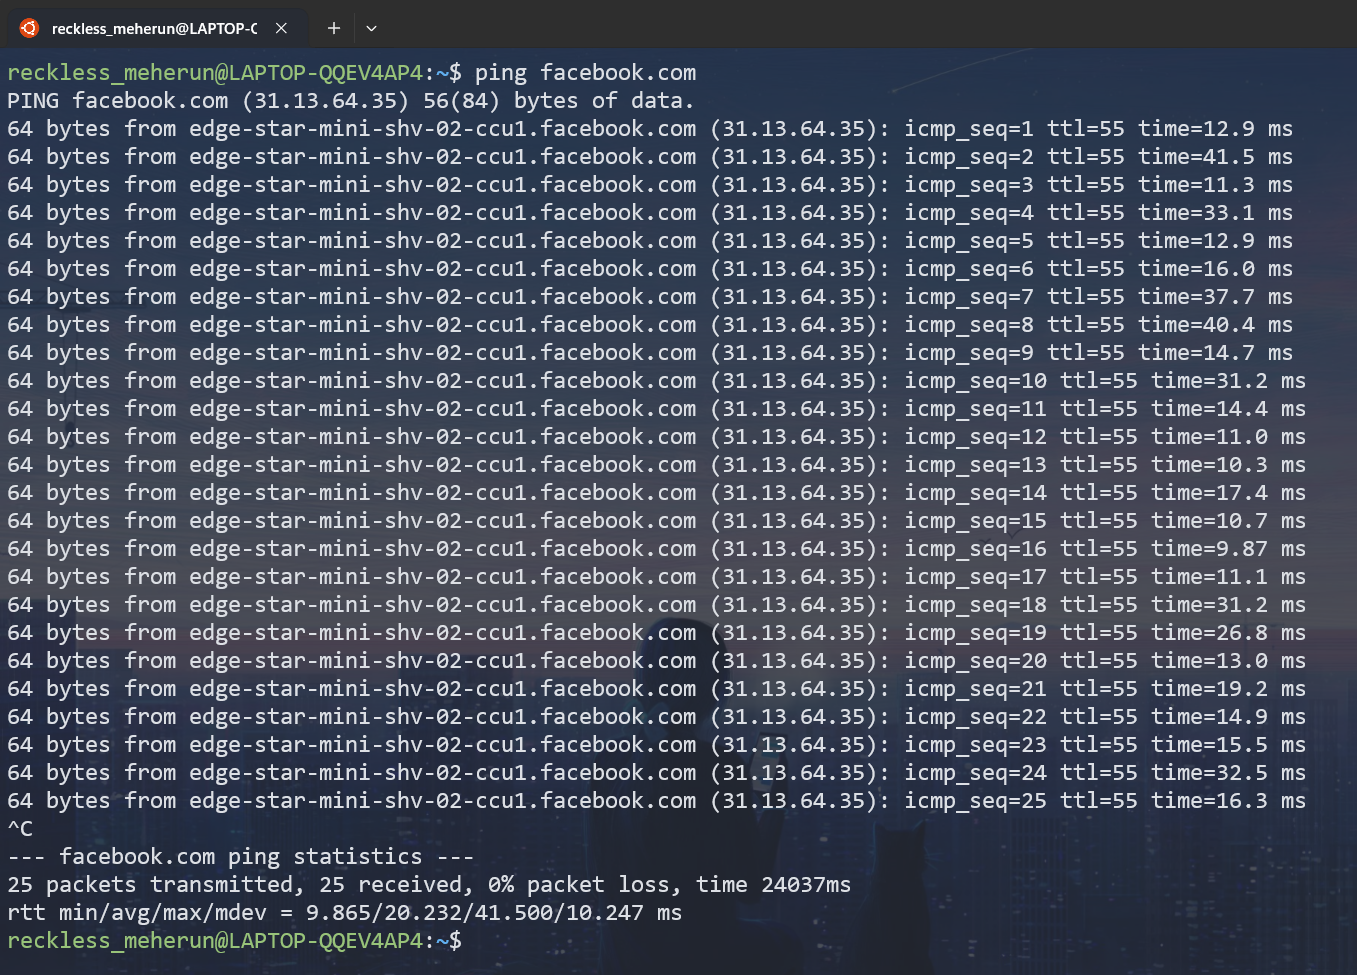
\includegraphics[width=\textwidth]{res/ping 1.png}
\caption{Sending ping to facebook}
\end{figure}

\subsubsection*{Limiting ping count}
\emph{-c} flag is used to fix the number of echo request to be sent in order to avoid sending infinite echo requests.
\begin{figure}[H]
\centering
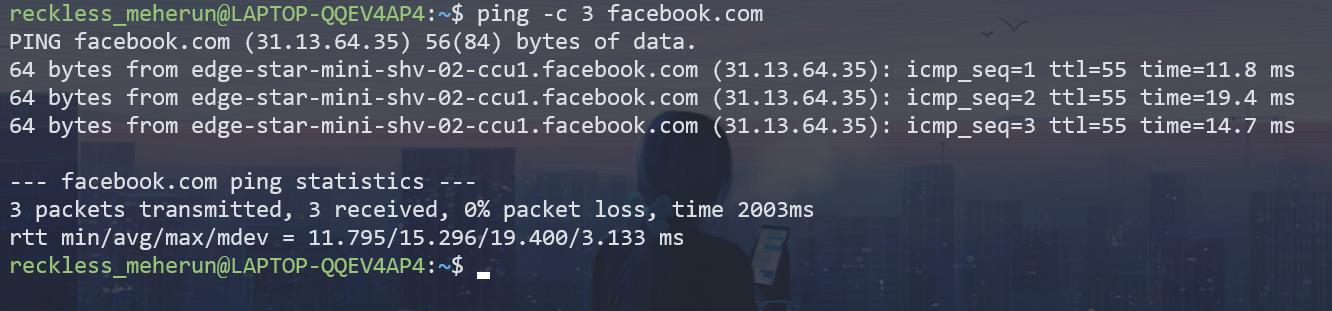
\includegraphics[width=\textwidth]{res/ping 2.png}
\caption{Limiting ping count to 3}
\end{figure}

\subsection{TRACEROUTE}
\begin{verbatim}
	traceroute youtube.com
\end{verbatim}
\begin{figure}[H]
\centering
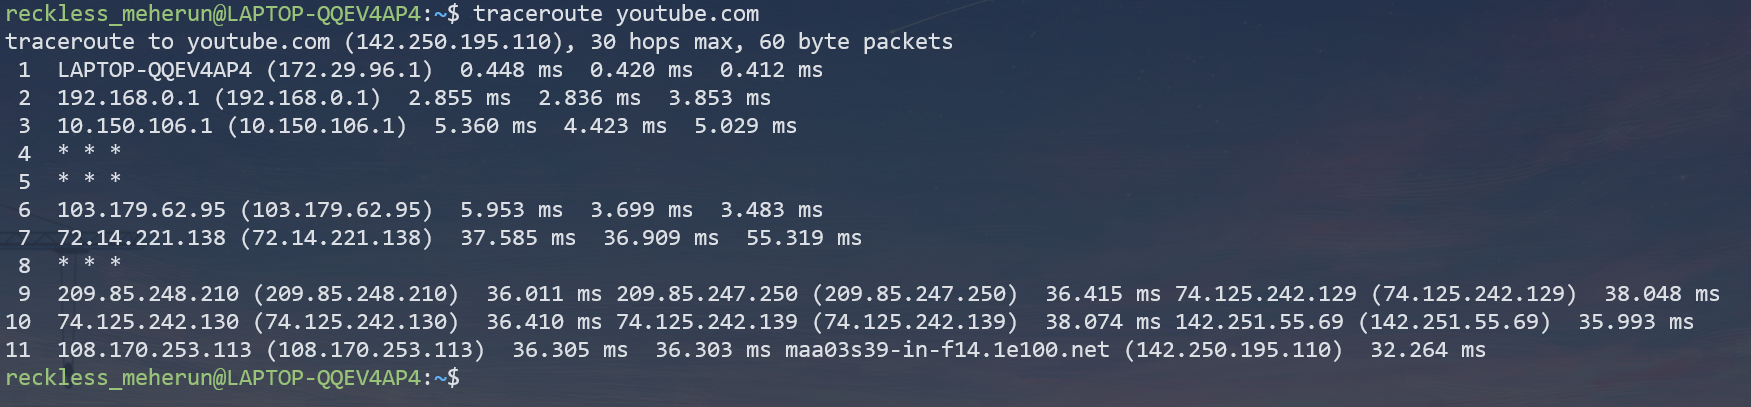
\includegraphics[width=\textwidth]{res/traceroute 1.png}
\caption{Tracking the route of a packet sent to youtube.com}
\end{figure}

\subsubsection*{Limiting maximum number of hops}
\emph{-m} flag is used to specify  the maximum number of hops (max time-to-live value) traceroute will probe. The default is 30.
\begin{figure}[H]
\centering
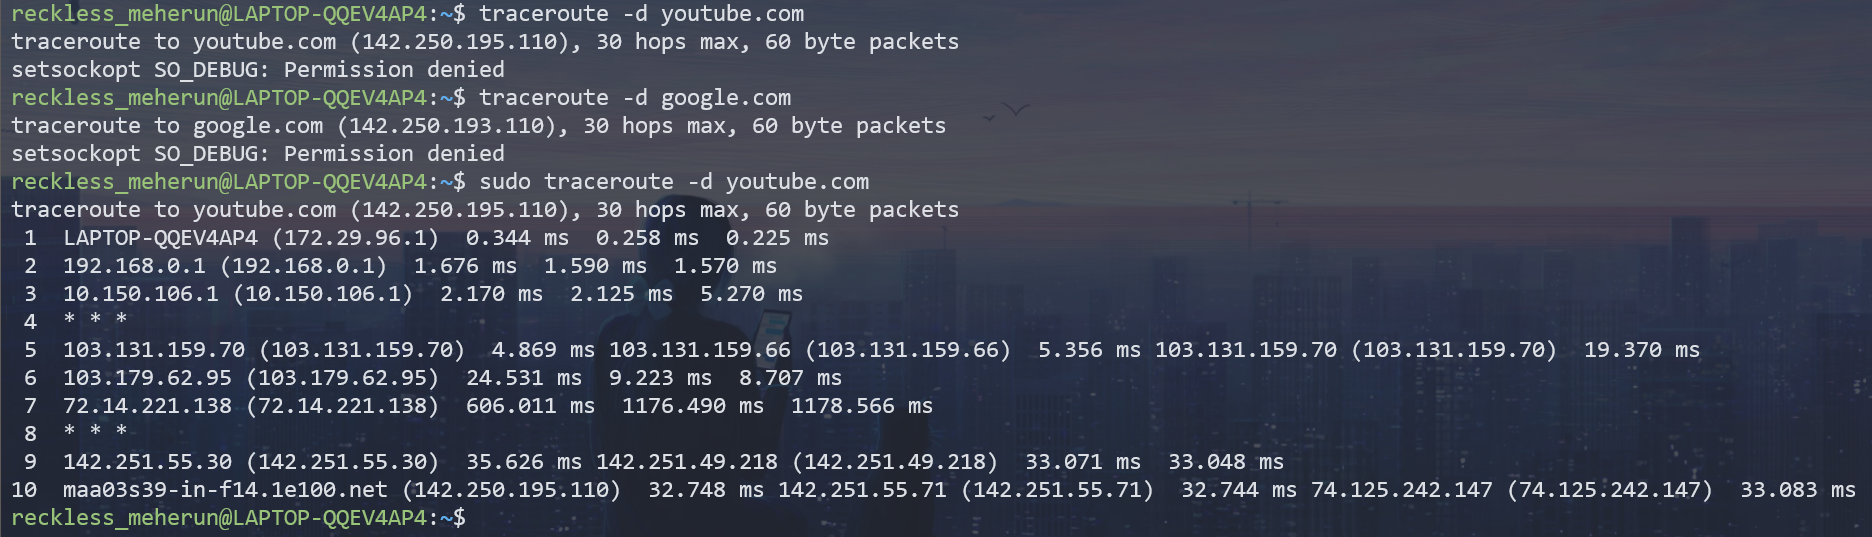
\includegraphics[width=\textwidth]{res/traceroute 2.png}
\caption{limiting maximum hop count to 3}
\end{figure}
\begin{figure}[H]
\centering
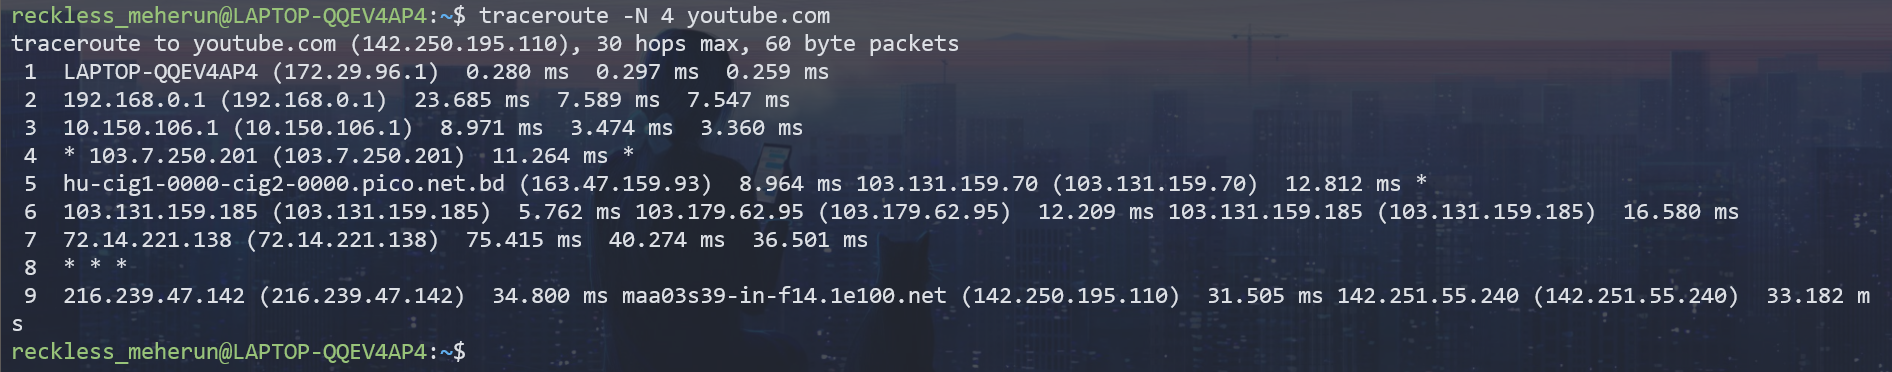
\includegraphics[width=\textwidth]{res/traceroute 3.png}
\end{figure}
\begin{figure}[H]
\centering
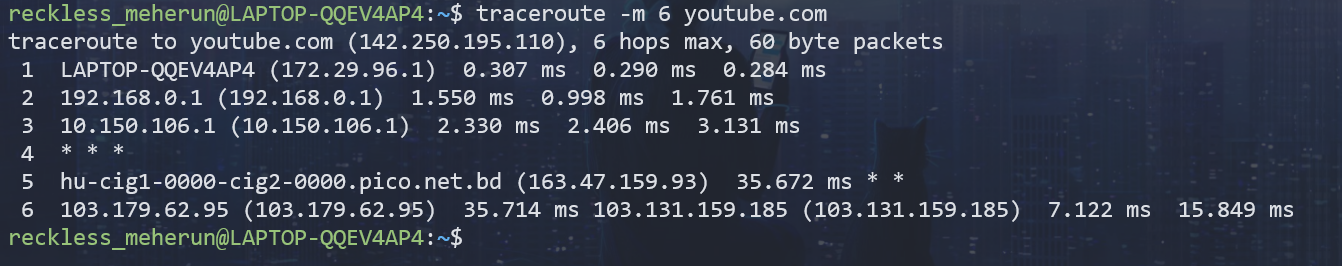
\includegraphics[width=\textwidth]{res/traceroute 4.png}
\end{figure}
\begin{figure}[H]
\centering
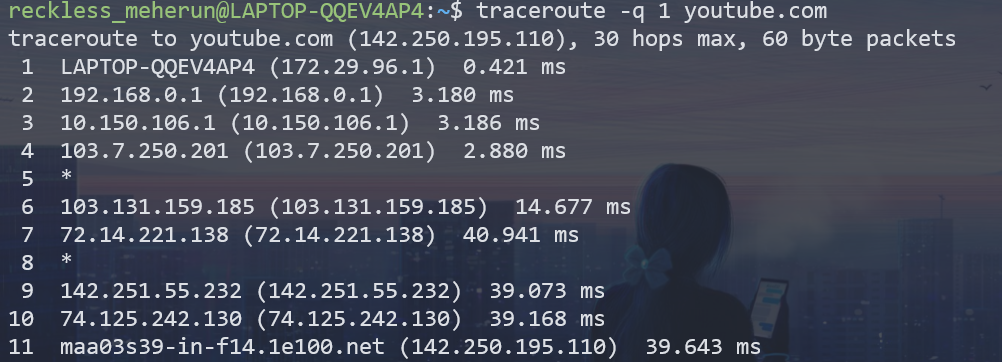
\includegraphics[width=\textwidth]{res/traceroute 5.png}
\end{figure}
\begin{figure}[H]
\centering
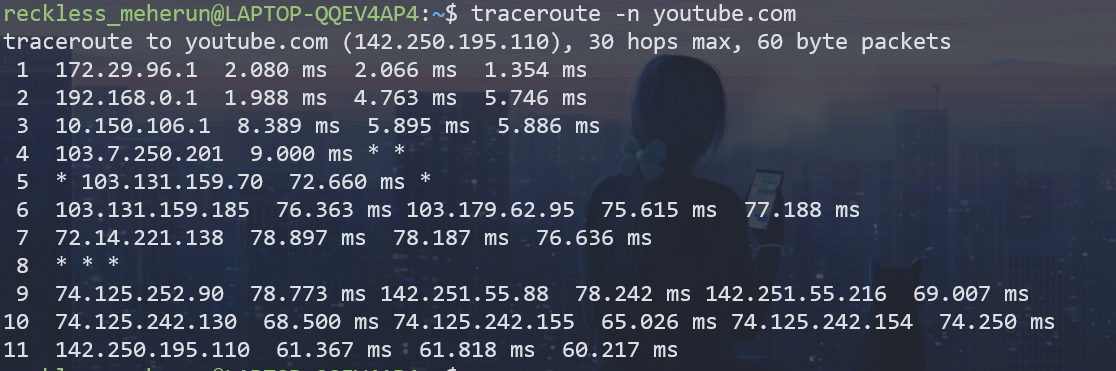
\includegraphics[width=\textwidth]{res/traceroute 6.png}
\end{figure}
\begin{figure}[H]
\centering
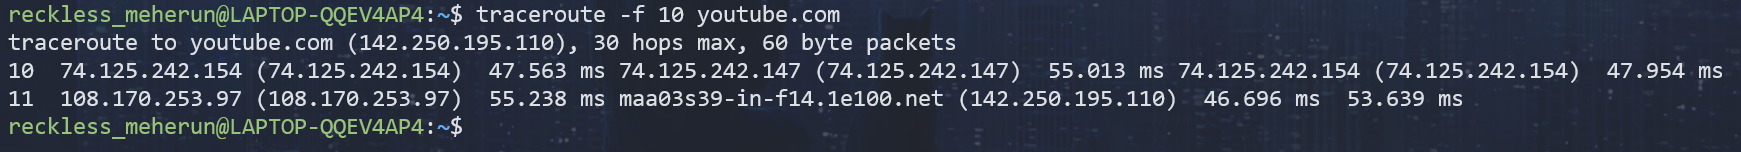
\includegraphics[width=\textwidth]{res/traceroute 7.png}
\end{figure}
\begin{figure}[H]
\centering
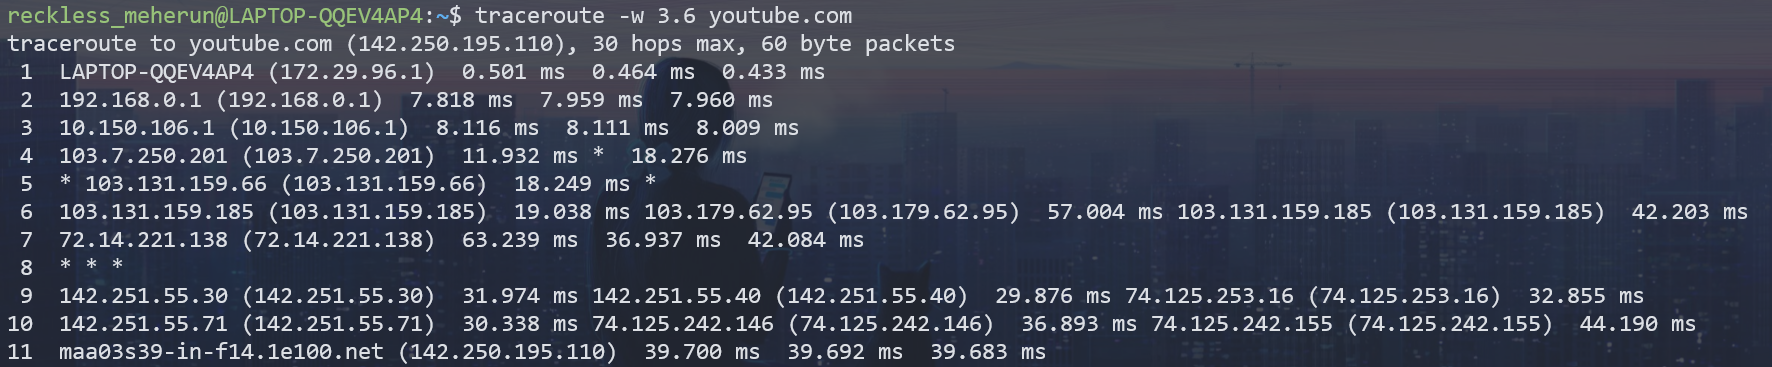
\includegraphics[width=\textwidth]{res/traceroute 8.png}
\end{figure}
\begin{figure}[H]
\centering
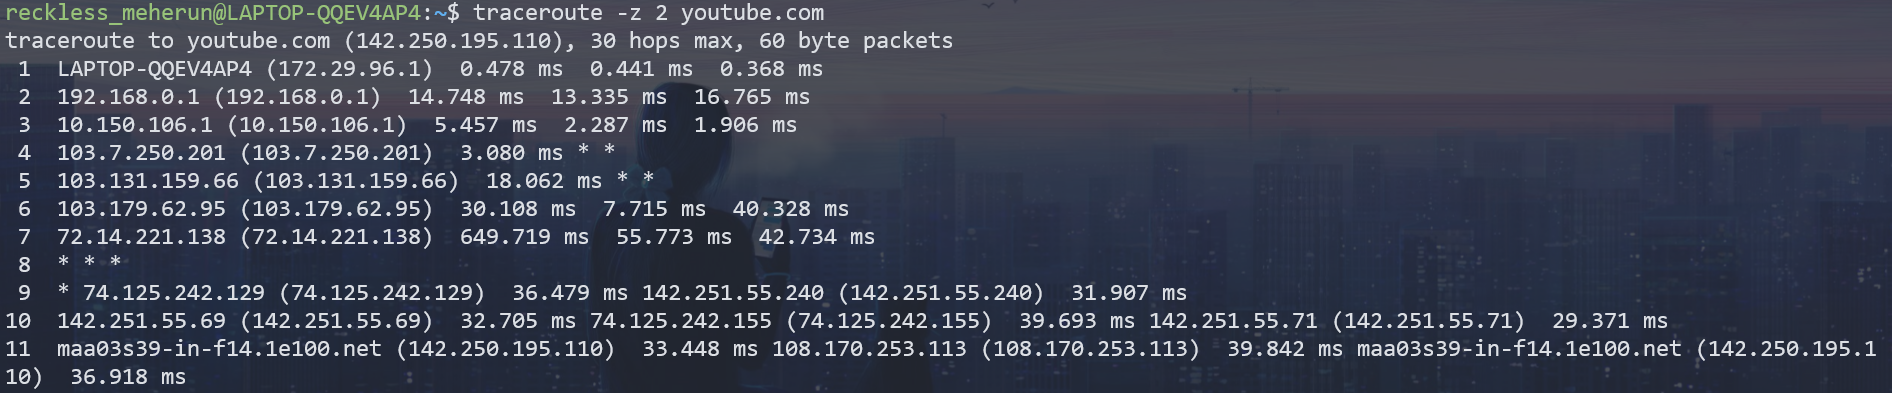
\includegraphics[width=\textwidth]{res/traceroute 9.png}
\end{figure}
\begin{figure}[H]
\centering
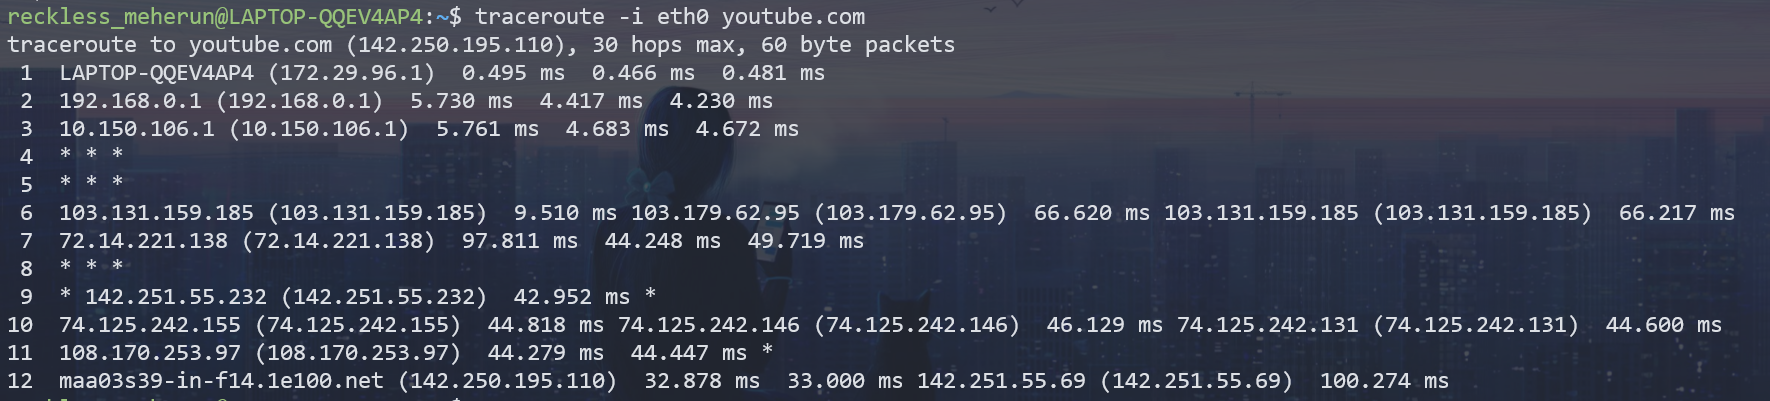
\includegraphics[width=\textwidth]{res/traceroute 10.png}
\end{figure}




\subsection{IFCONFIG}
\begin{verbatim}
	ifconfig
\end{verbatim}
\begin{figure}[H]
\centering
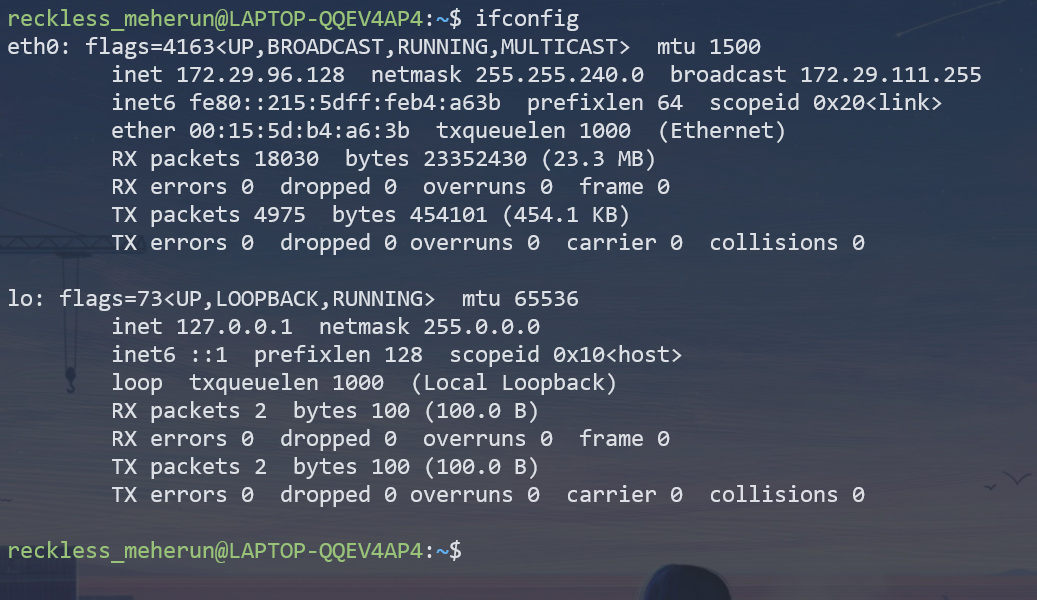
\includegraphics[width=\textwidth]{res/ifconfig 1.png}
\caption{Getting currently active interfaces information using ifconfig}
\end{figure}

\subsubsection*{Getting all interfaces}
\emph{-a} flag is to display all interfaces which are currently available, even if down.
\begin{figure}[H]
\centering
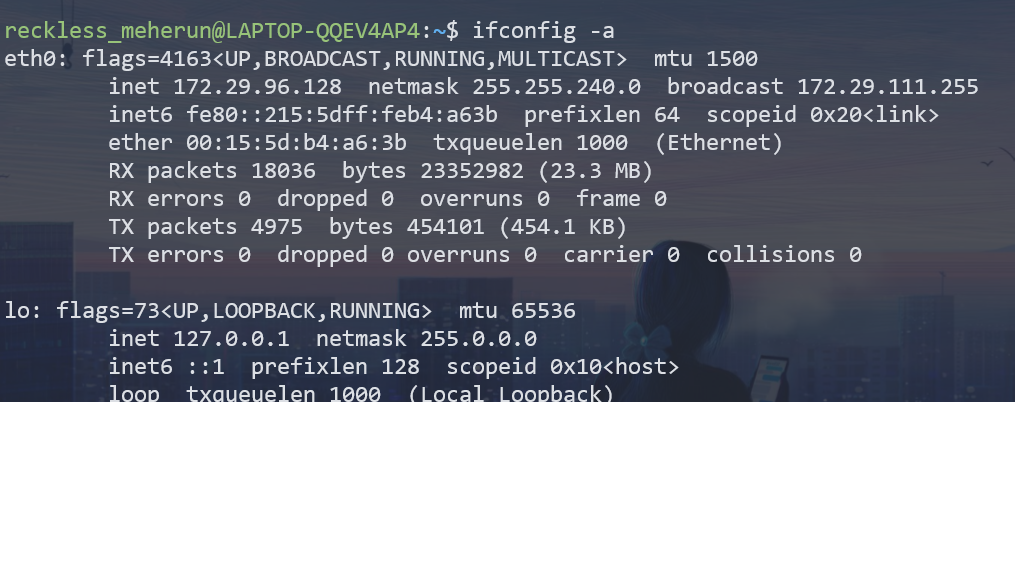
\includegraphics[width=\textwidth]{res/ifconfig 2.png}
\caption{Getting all interfaces}
\end{figure}

\subsubsection*{Specifying an interface}
Providing the name of an interface shows information about that only.
\begin{figure}[H]
\centering
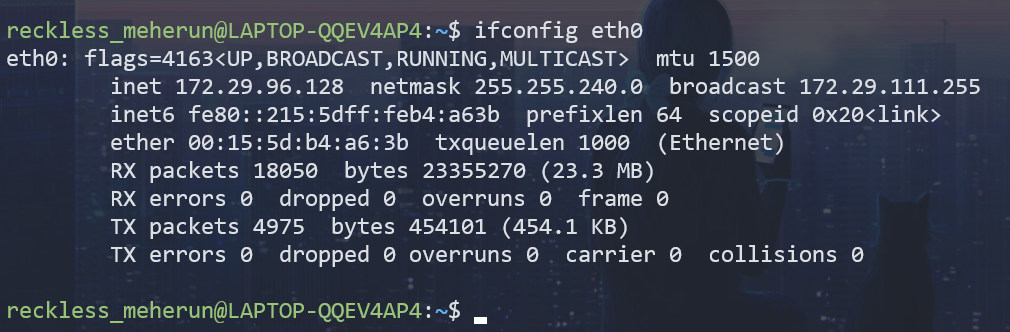
\includegraphics[width=\textwidth]{res/ifconfig 3.png}
\caption{Getting information of eth0 interface}
\end{figure}

\subsubsection*{Activating an interface}
\emph{up} is used to activate an interface.
\begin{figure}[H]
\centering

\includegraphics[width=\textwidth]{res/ifconfig 4.png}
\caption{Activating eth0}
\end{figure}

\subsection{ARP}
\begin{verbatim}
	arp
\end{verbatim}
\begin{figure}[H]
\centering
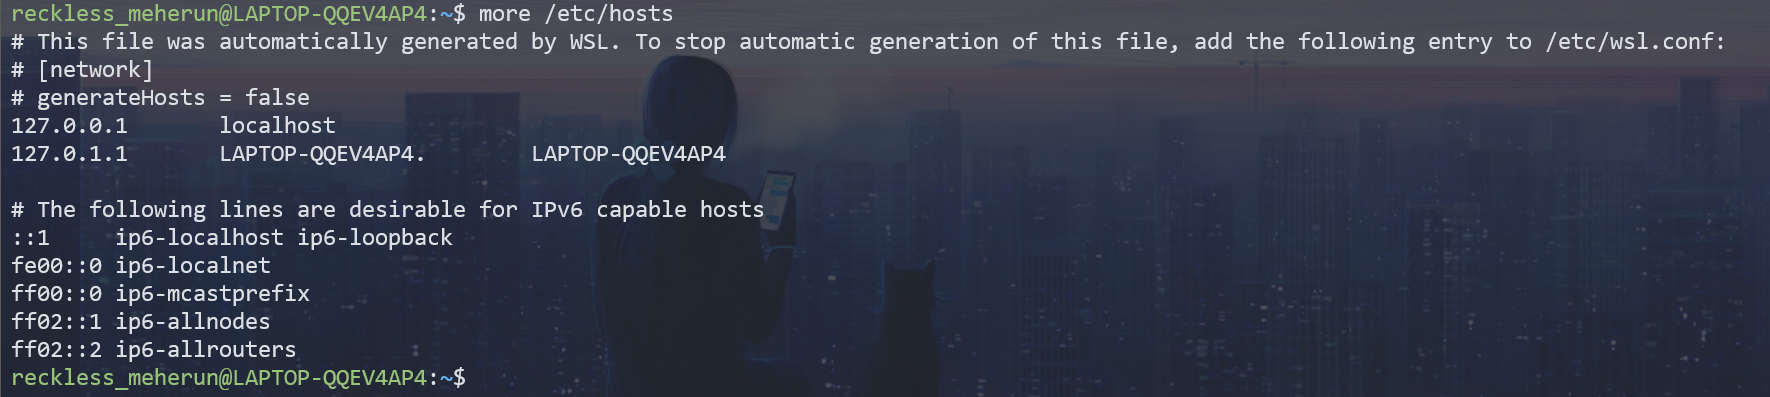
\includegraphics[width=\textwidth]{res/arp 1.png}
\caption{Showing the current table content}
\end{figure}

\subsubsection*{Verbose}
\emph{-V} flag provides a more verbose description.
\subsubsection*{Numeric address}
\emph{-n} flag shows numeric addresses instead of symbolic names
\begin{figure}[H]
\centering
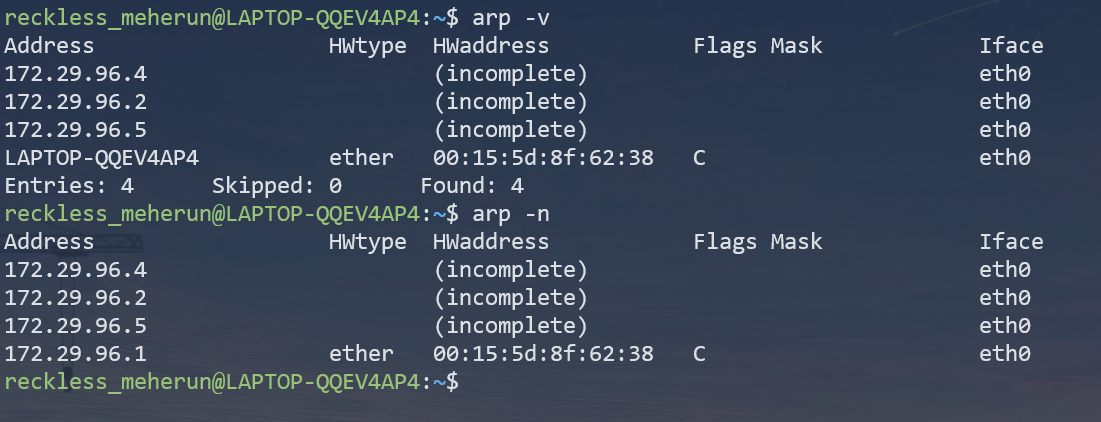
\includegraphics[width=\textwidth]{res/arp 2.png}
\caption{Different arp flags}
\end{figure}

\subsection{RARP}
\begin{verbatim}
	rarp
\end{verbatim}
\begin{figure}[H]
\centering
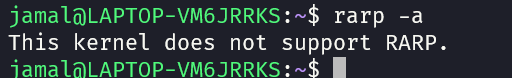
\includegraphics[width=\textwidth]{res/rarp 1.png}
\caption{RARP not usable for being outdated}
\end{figure}

\subsection{NSLOOKUP}
\begin{verbatim}
	traceroute youtube.com
\end{verbatim}
\begin{figure}[H]
\centering
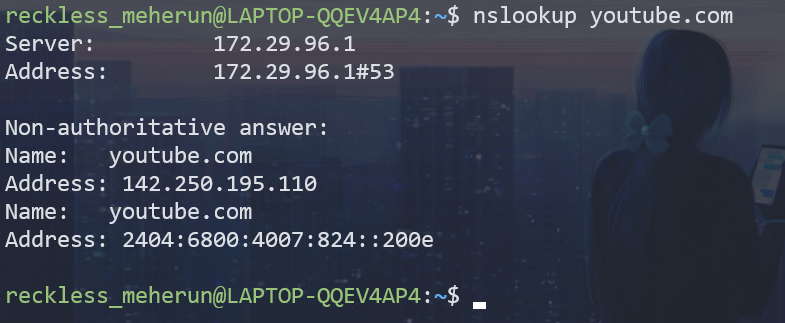
\includegraphics[width=\textwidth]{res/nslookup 1.png}
\caption{Printing the name and requested information for a youtube.com.}
\end{figure}

\subsubsection*{View all available records.}
\emph{-type=any} flag is used to view all available records about the host. We can also specify what type of information we want.
\begin{figure}[H]
\centering
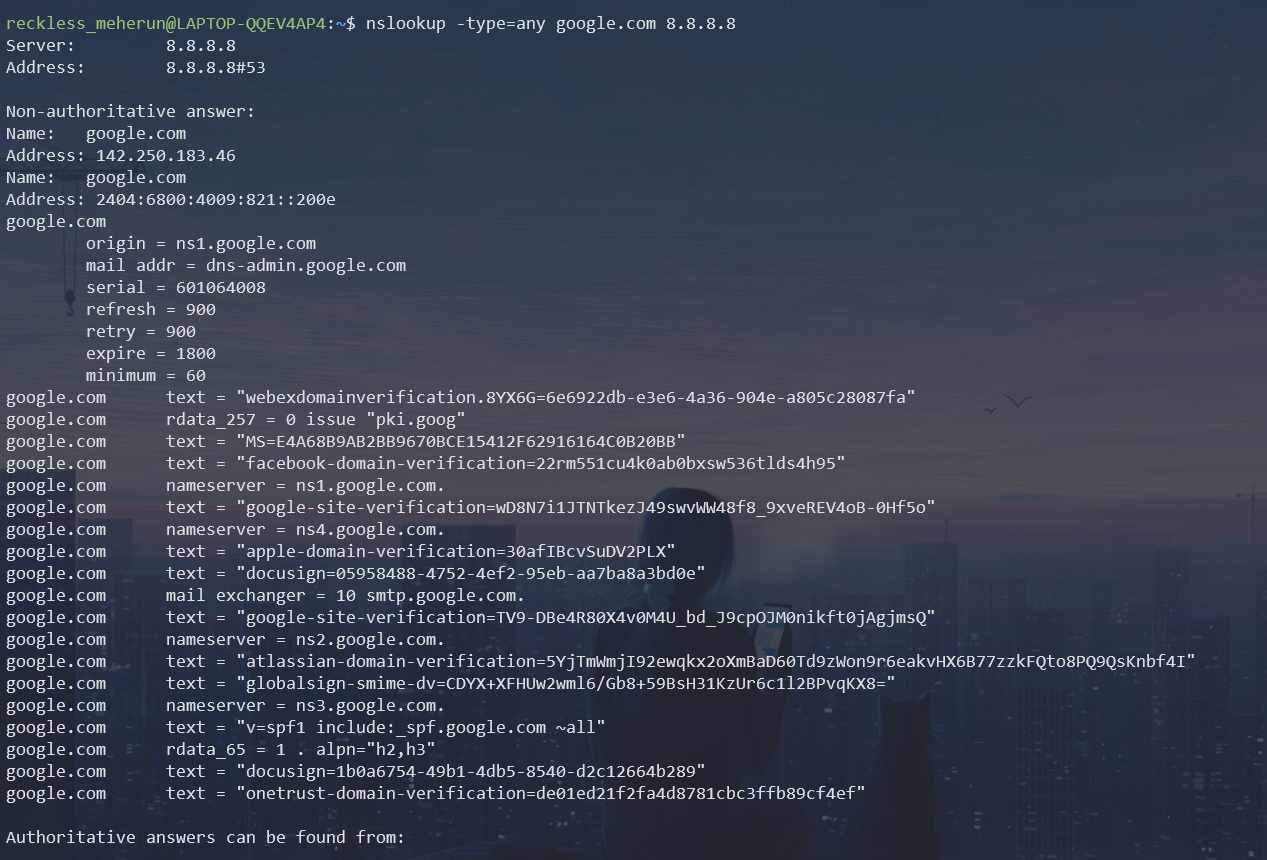
\includegraphics[width=\textwidth]{res/nslookup 3.png}
\caption{View all available records of youtube.com}
\end{figure}
\begin{figure}[H]
\centering
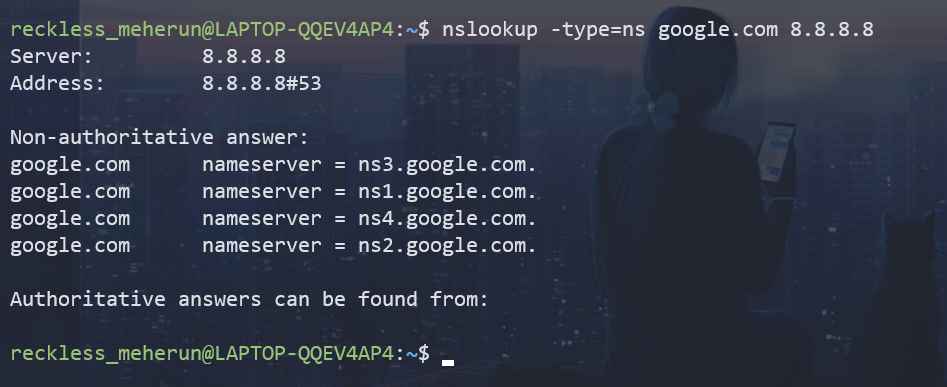
\includegraphics[width=\textwidth]{res/nslookup 4.png}
\caption{View name server records of youtube.com}
\end{figure}
\begin{figure}[H]
\centering
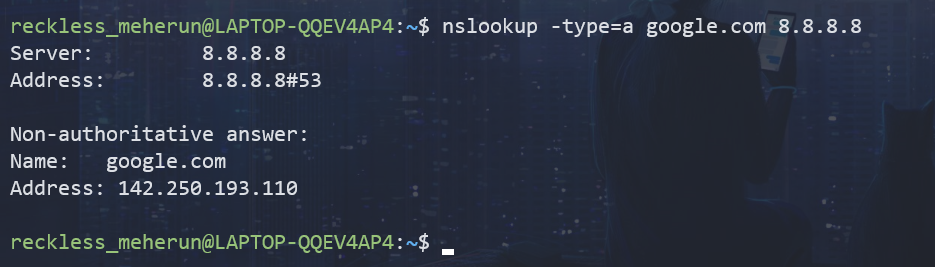
\includegraphics[width=\textwidth]{res/nslookup 5.png}
\caption{View DNS A address records of youtube.com}
\end{figure}
\begin{figure}[H]
\centering
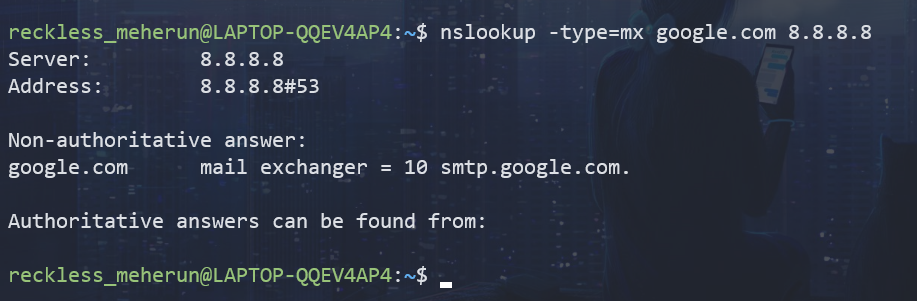
\includegraphics[width=\textwidth]{res/nslookup 6.png}
\caption{View mail exchange records of youtube.com}
\end{figure}
\begin{figure}[H]
\centering
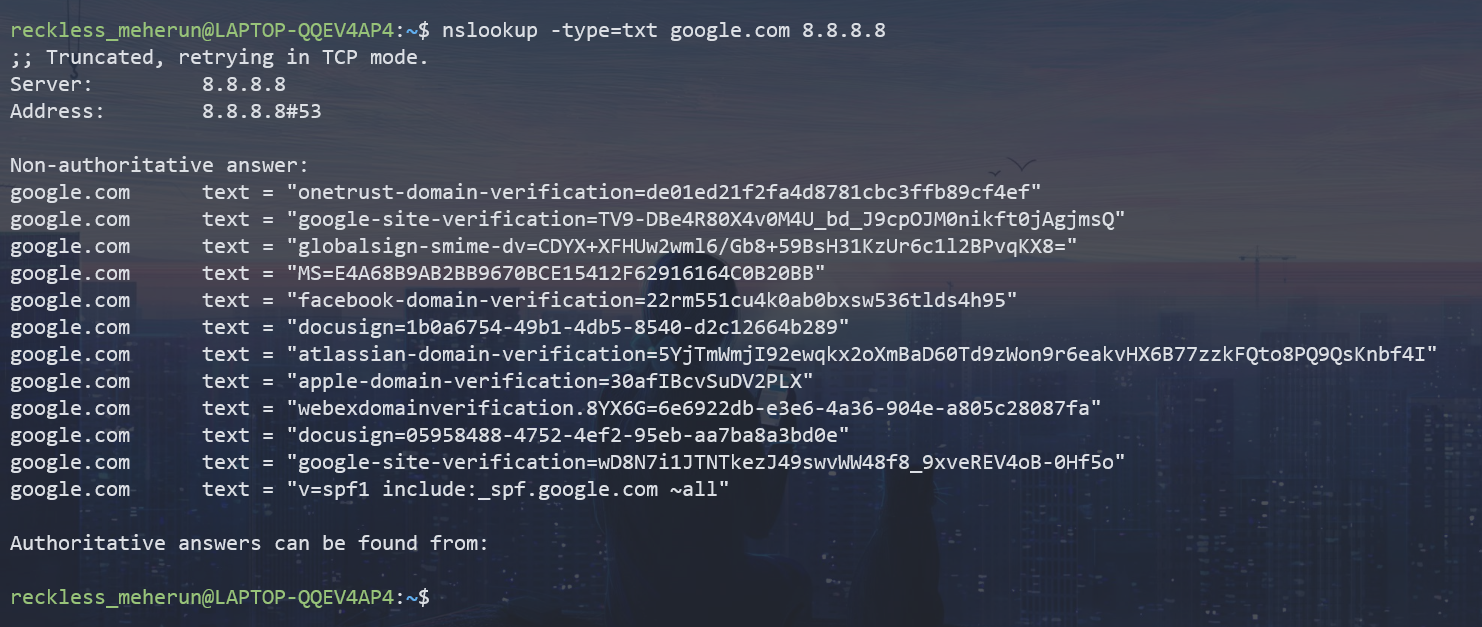
\includegraphics[width=\textwidth]{res/nslookup 7.png}
\caption{View txt records of youtube.com}
\end{figure}

\subsection{NETSTAT}
\begin{verbatim}
	netstat
\end{verbatim}

\begin{figure}[H]
	\centering
	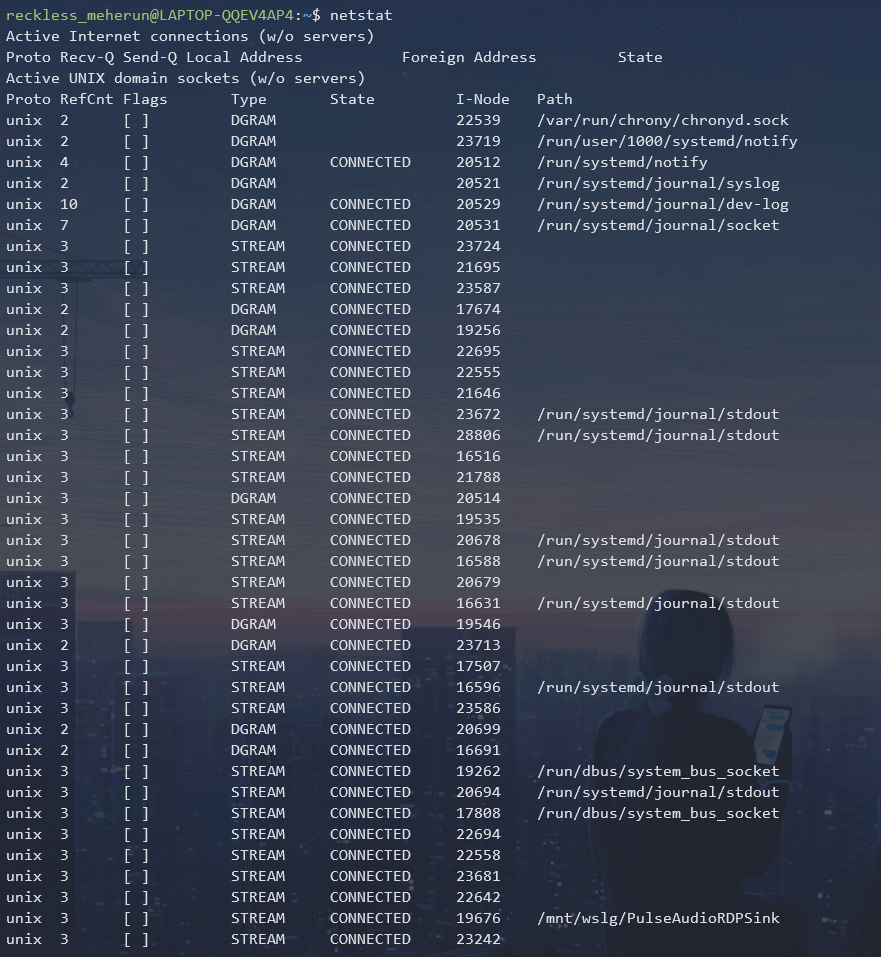
\includegraphics[width=\textwidth]{res/netstat 1.png}
	\caption{Displaying all open sockets}
\end{figure}
\begin{figure}[H]
	\centering
	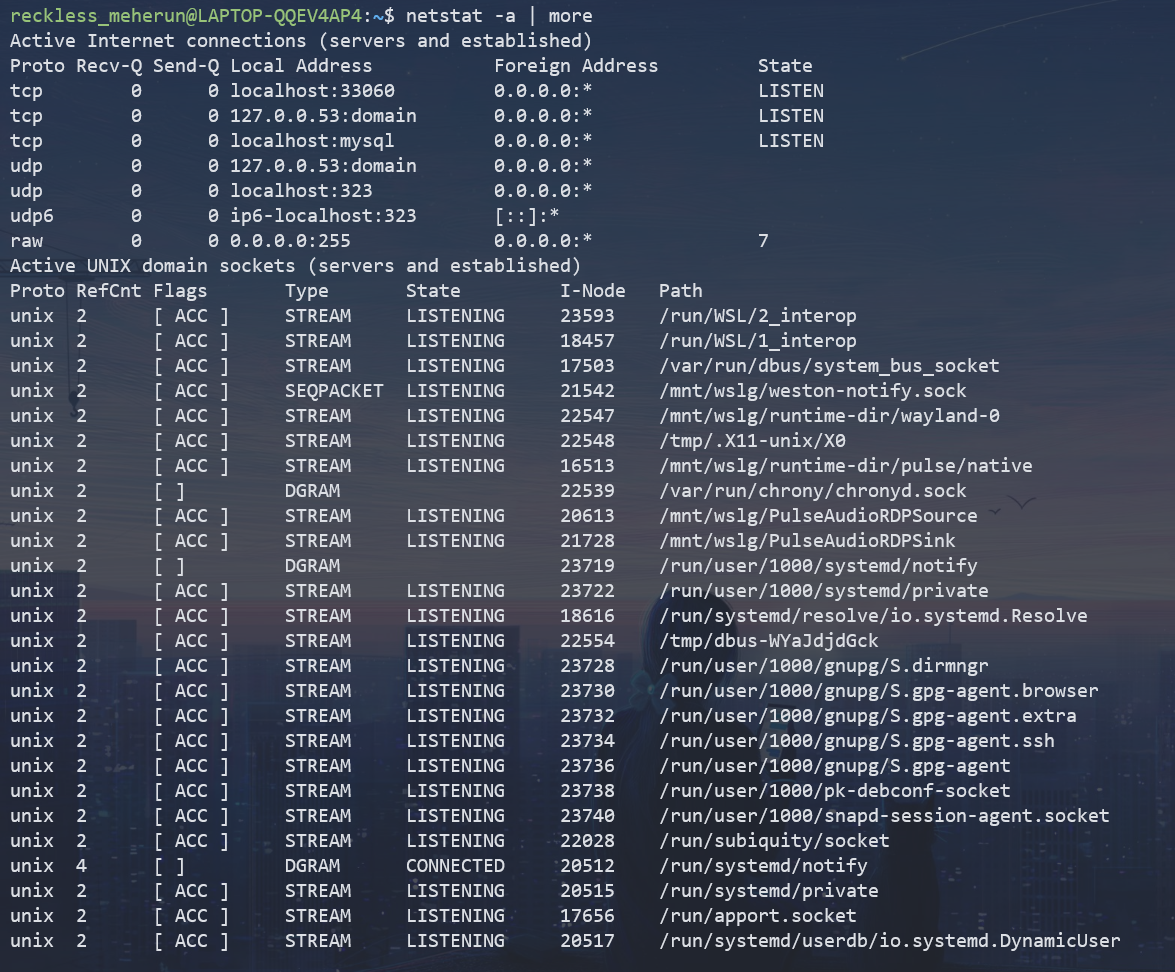
\includegraphics[width=\textwidth]{res/netstat 2.png}
	\caption{Showing all listening and non listening ports}
\end{figure}
\begin{figure}[H]
	\centering
	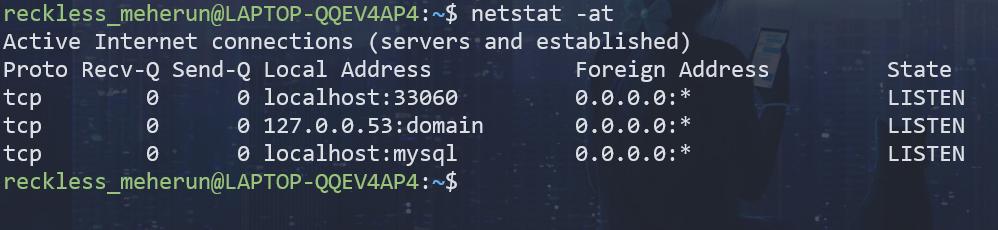
\includegraphics[width=\textwidth]{res/netstat 3.png}
	\caption{Showing all tcp sockets}
\end{figure}
\begin{figure}[H]
	\centering
	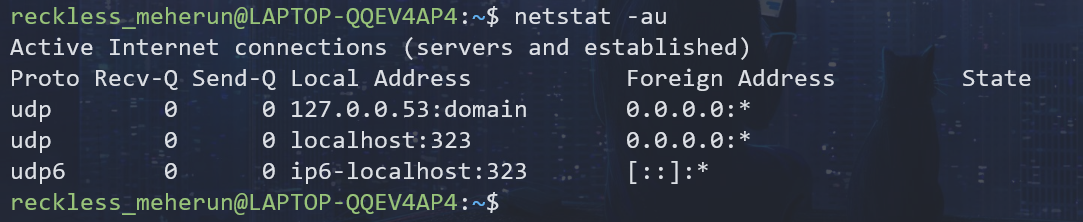
\includegraphics[width=\textwidth]{res/netstat 4.png}
	\caption{Showing all udp sockets}
\end{figure}
\begin{figure}[H]
	\centering
	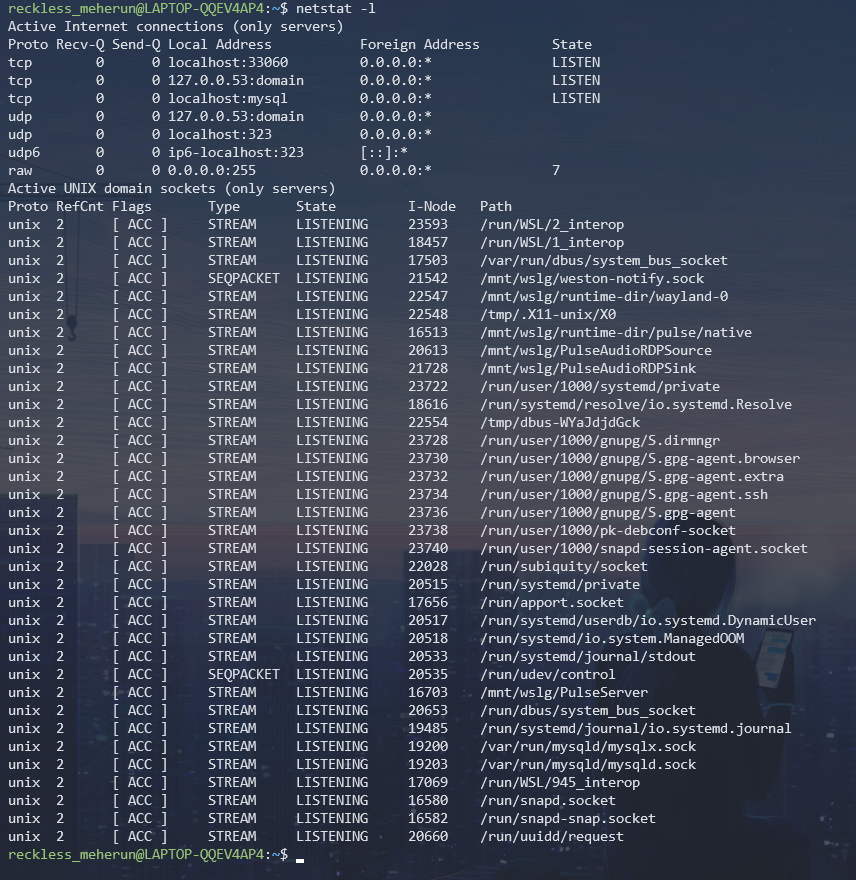
\includegraphics[width=\textwidth]{res/netstat 5.png}
	\caption{Showing only listening sockets}
\end{figure}
\begin{figure}[H]
	\centering
	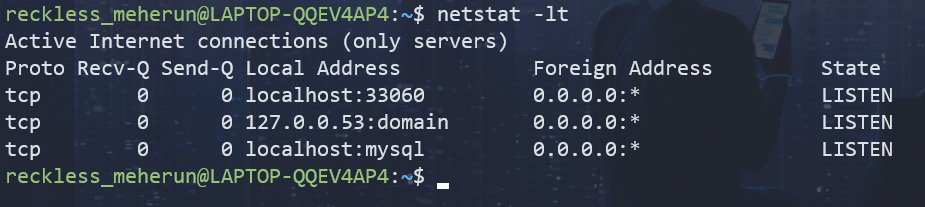
\includegraphics[width=\textwidth]{res/netstat 6.png}
	\caption{Showing listening tcp sockets}
\end{figure}
\begin{figure}[H]
	\centering
	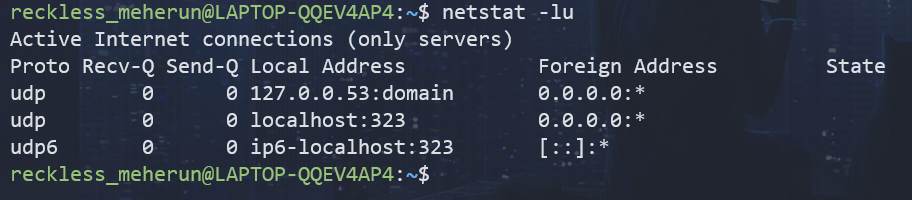
\includegraphics[width=\textwidth]{res/netstat 7.png}
	\caption{Showing listening udp sockets}
\end{figure}
\begin{figure}[H]
	\centering
	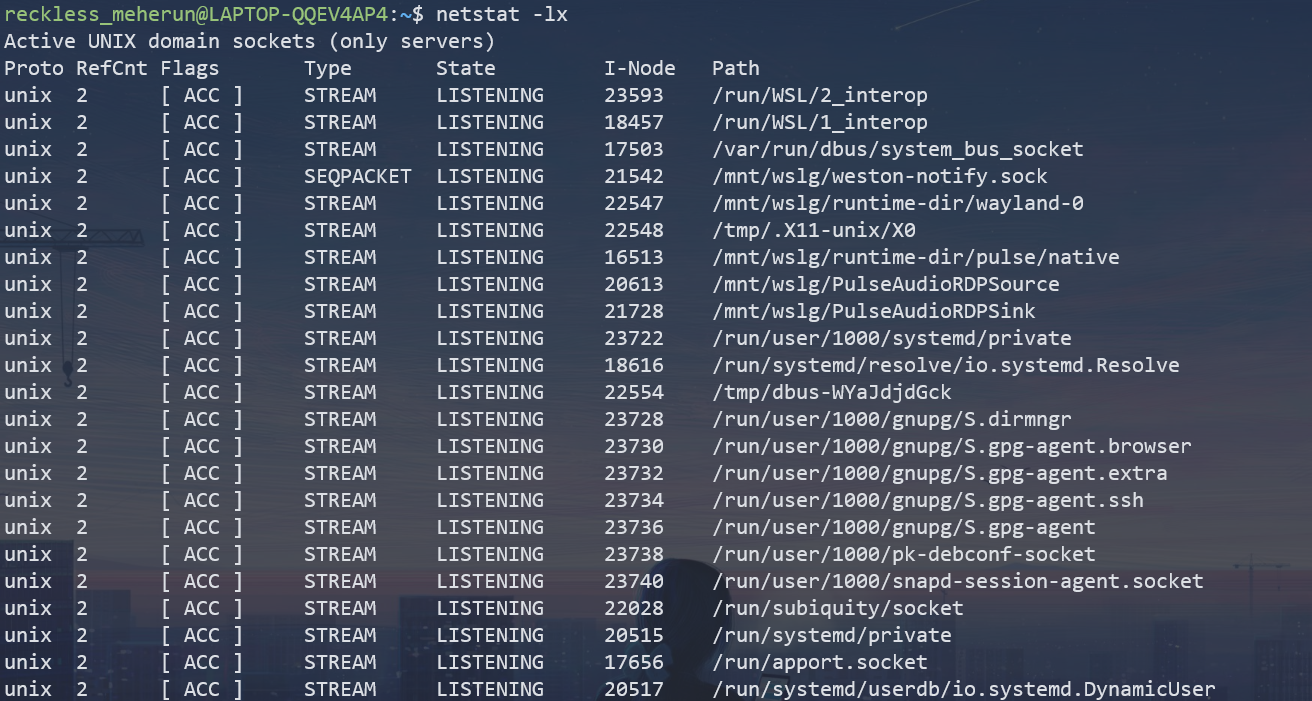
\includegraphics[width=\textwidth]{res/netstat 8.png}
	\caption{Showing listening unix sockets}
\end{figure}
\begin{figure}[H]
	\centering
	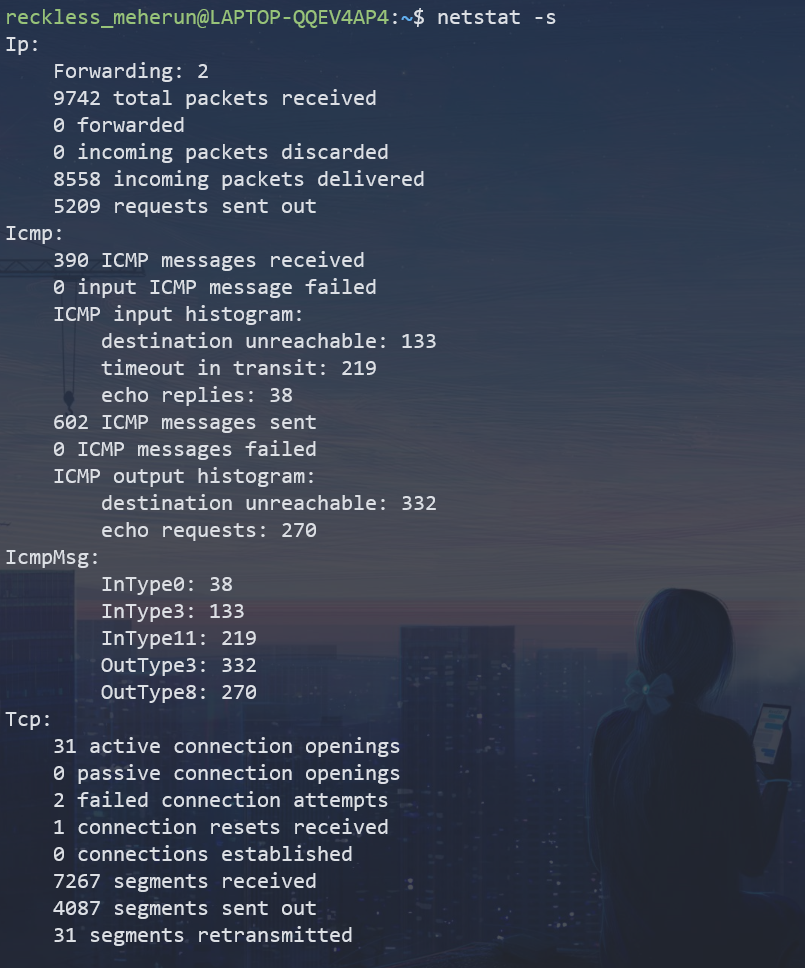
\includegraphics[width=\textwidth]{res/netstat 9.png}
	\caption{Displaying summary statistics for each protocol.}
\end{figure}
\begin{figure}[H]
	\centering
	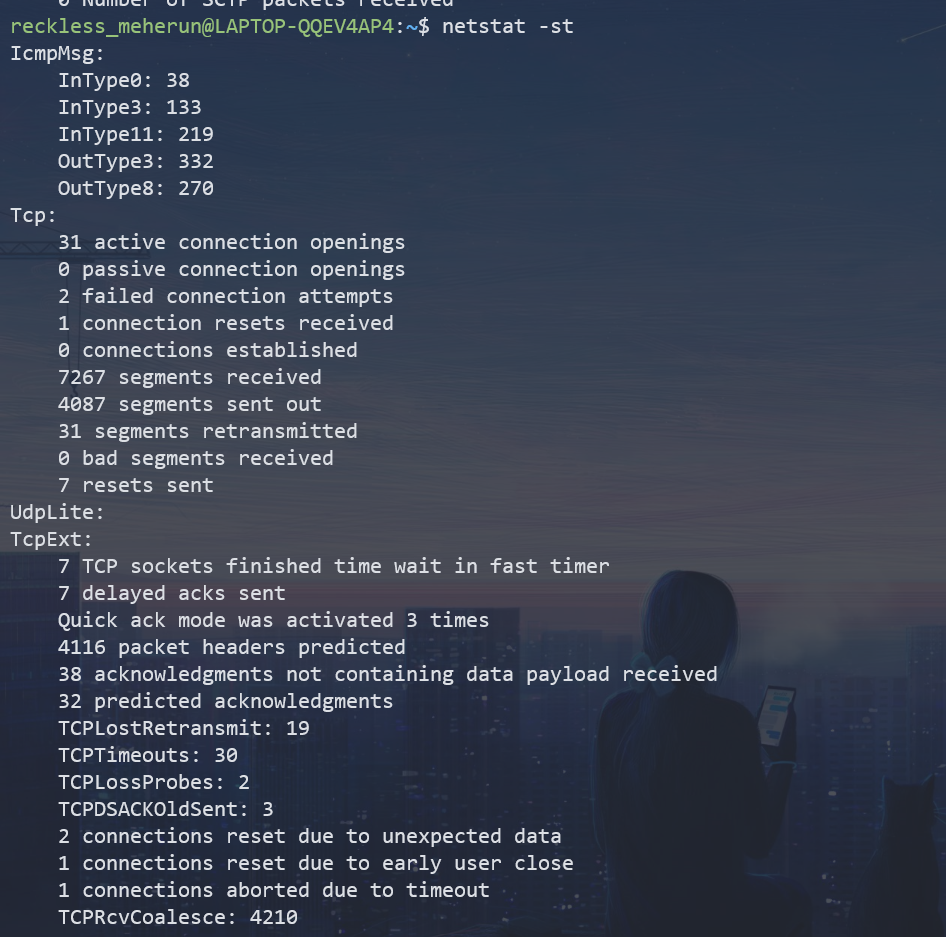
\includegraphics[width=\textwidth]{res/netstat 10.png}
	\caption{Displaying summary statistics for tcp protocol.}
\end{figure}
\begin{figure}[H]
	\centering
	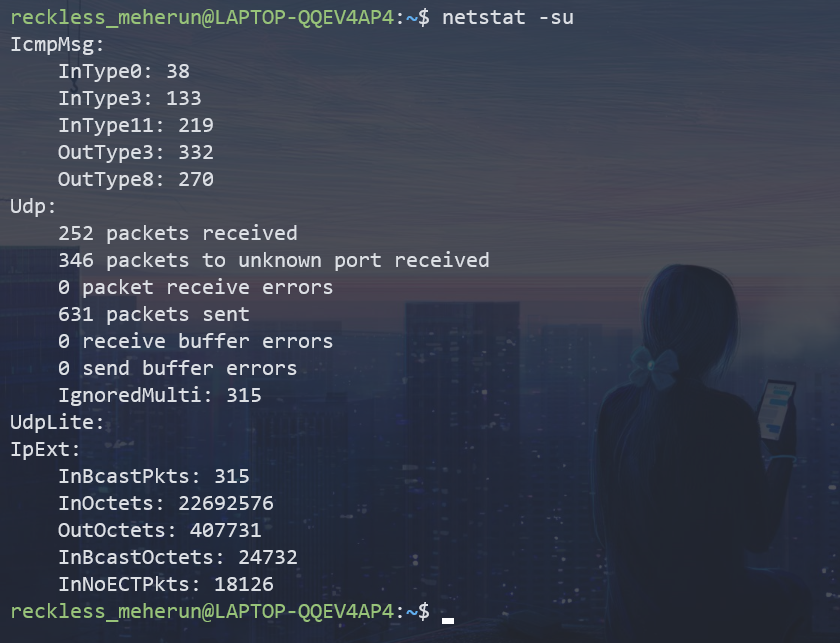
\includegraphics[width=\textwidth]{res/netstat 11.png}
	\caption{Displaying summary statistics for udp protocol.}
\end{figure}
\begin{figure}[H]
	\centering
	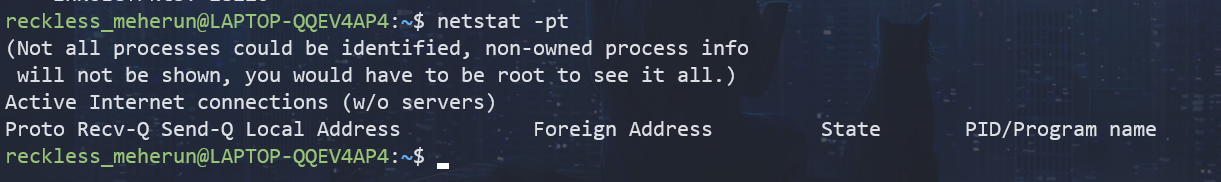
\includegraphics[width=\textwidth]{res/netstat 12.png}
	\caption{Show the PID and name of the program to which tcp sockets belong.}
\end{figure}
\begin{figure}[H]
	\centering
	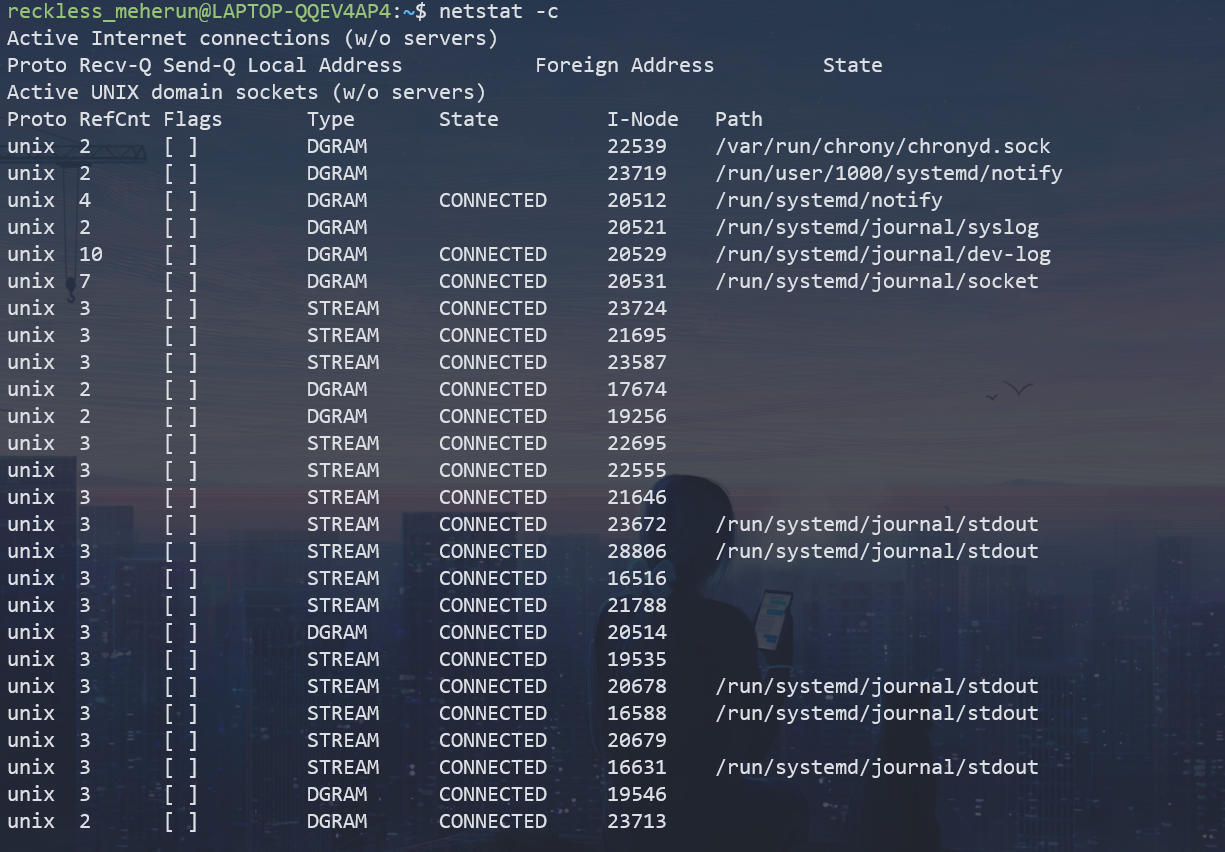
\includegraphics[width=\textwidth]{res/netstat 13.png}
	\caption{Printing the selected information every second continuously}
\end{figure}
\begin{figure}[H]
	\centering
	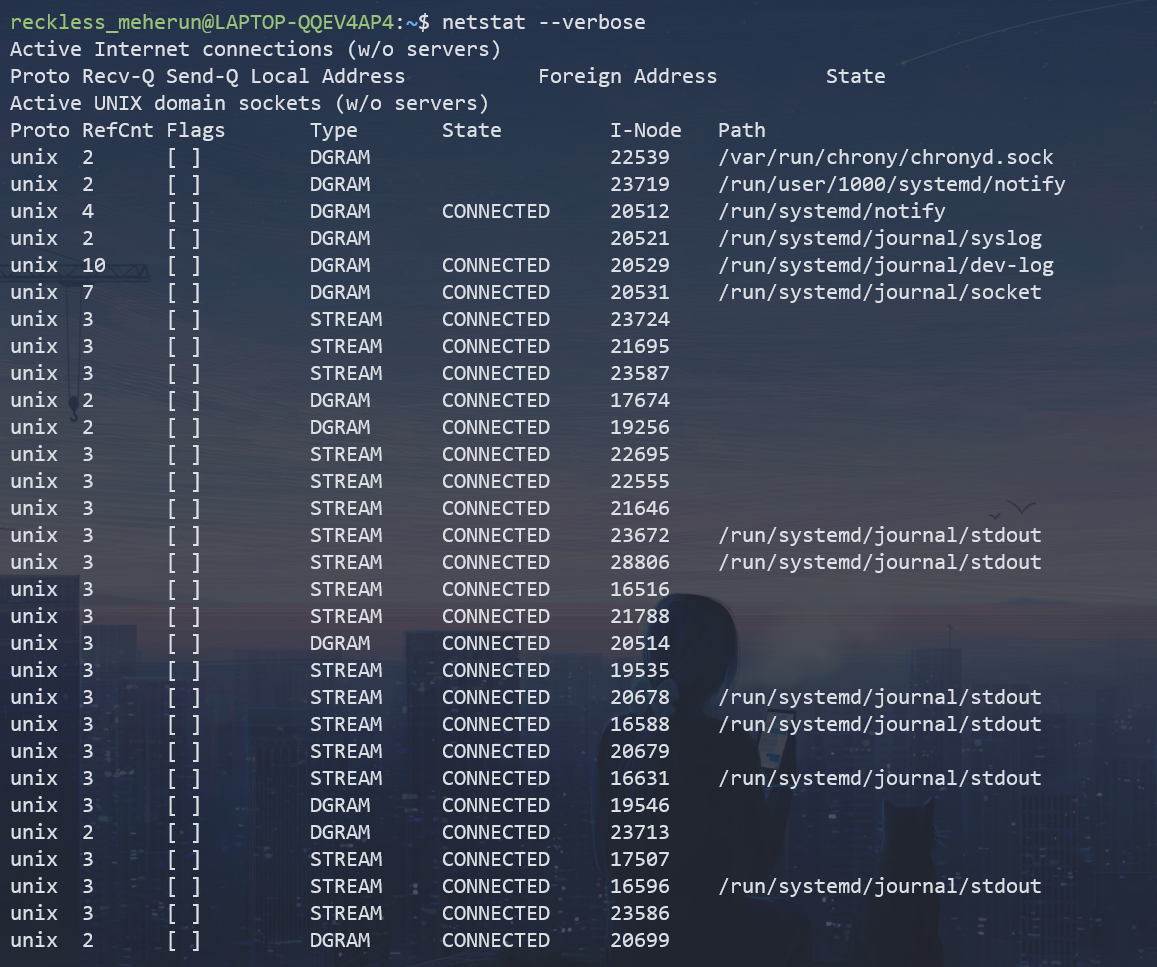
\includegraphics[width=\textwidth]{res/netstat 14.png}
	\caption{Telling the user what is going on by being verbose}
\end{figure}
	

\newpage
\section{Experience}
\begin{enumerate}
\item We learned how to utilized troubleshooting tools including PING, Traceroute, ARP, and netstat to diagnose and resolve connectivity issues.
\item We used ifconfig to manage network interfaces and nslookup for DNS-related problem-solving..
\end{enumerate}

\begin{thebibliography}{1}
\bibitem{book}  Computer networking: a top-down approach 6th ed.
\bibitem{PING} PING: \url{https://pimylifeup.com/ubuntu-
ping/#:~:text=Example%20of%20Limiting%20the%20Number%20of%20pings%20on%20Ubuntu&amp;text=T
o%20achieve%20this%2C%20we%20use,the%20destination%20for%20our%20pings.&amp;text=After%20run
ning%20this%20command%2C%20your,to%20stop%20the%20process%20manually.
}
\bibitem{TRACEROUTE} TRACEROUTE: \url{https://cloudinfrastructureservices.co.uk/how-to-install-traceroute-and-run-on-ubuntu-20-04/}
\bibitem{IFCONFIG} IFCONFIG: \url{https://www.tecmint.com/ifconfig-command-examples/}
\bibitem{ARP} ARP: \url{https://www.geeksforgeeks.org/arp-command-in-linux-with-examples/}
\bibitem{RARP} RARP: \url{https://www.geeksforgeeks.org/what-is-rarp/}
\bibitem{NSLOOKUP} NSLOOKUP: \url{https://www.geeksforgeeks.org/nslookup-command-in-linux-with-examples/}
\bibitem{NETSTAT} NETSTAT: \url{https://www.geeksforgeeks.org/nslookup-command-in-linux-with-examples/}
\bibitem{NSLOOKUP} NSLOOKUP: \url{https://www.geeksforgeeks.org/netstat-command-linux//}
\bibitem{MindMajix} MindMajix: \url{https://mindmajix.com/linux-networking-commands-best-examples}
\end{thebibliography}

\end{document}